\section{Analysis and Discussion}
\label{sec:propwork-casod-disc}

%{\color{red}experiments or results comparing casod to prev methods?}

%\subsection{Parameter Cost and Runtime Analysis Details}
%\label{sec:suppmat-runtime}

%\textbf{Parameter Cost of \sys}. \sys uses a \textit{frozen} pre-trained ViT-B-16, only requiring the LoRA and FF components to be trained. \sys parameter efficiency improves over fully fine-tuning a multi-view model by \textbf{81\%} and over fully fine-tuning a single ViT backbone by \textbf{44\%}. {\color{blue}Additional memory comparisons are in Appendix Sec. C.3.} %{\color{red}memory and walltime cost during training - probably put in Appendix} {\color{blue}The \sys model alone consumes 36.68 MiB while the single-view baseline model consumes 2.67 MiB. Under our training settings (i.e. batch size of 128), \sys consumes 52.54 GiB of memory per GPU while a single-view baseline consumes 13.67 GiB. One epoch of training required 169 seconds walltime for \sys and 51 seconds walltime for a single-view baseline. These values scale as expected with batch size. With a batch size of 64, \sys consumes 26.27 GiB and 181 seconds walltime while a single-view baseline consumes 8.19 GiB and 54 seconds walltime.}
%
%\textbf{Parameter Cost - Details}. As mentioned in the main paper, \sys uses a \textit{frozen} pre-trained ViT-B-16 as a feature extractor and only requires the LoRA modules and feature fusion component to be trained. The standard multi-view classification technique of training separate backbones for each view requires about 259 million (M) trainable parameters for three views. \sys only requires 48 M trainable parameters for three views, a parameter efficiency improvement of \textbf{81\%}. \sys also improves over fully fine-tuning a single ViT backbone which involves 86 M trainable parameters, an efficiency improvement of \textbf{44\%}.
%
%{\color{blue}We profiled \sys and a single-view baseline model for comparison. The \sys model alone consumes 36.68 MiB while the single-view baseline model consumes 2.67 MiB. Training \sys with a batch size of 128 consumes 52.54 GiB of memory per GPU while a single-view baseline consumes 13.67 GiB. These values scale as expected with batch size. With a batch size of 64, \sys consumes 26.27 GiB while a single-view baseline consumes 8.19 GiB.}
\subsection{Complexity Details}
\label{sec:casod_suppmat-runtime}

\subsubsection{Parameter Cost}
As \gls{sys} is designed around a frozen pre-trained ViT-B-16 model architecture, the only trainable parameters are in the LoRA and fusion components, cumulatively amounting to 48 million (M) trainable parameters for three views. When compared to a fully fine-tuned multi-view model, which amounts to a total of 259 M trainable parameters for three views, \gls{sys} improves parameter efficiency by 81\%. When compared to a fully fine-tuned model using a single ViT backbone feature extractor, which amounts to a total of 86 M trainable parameters, \gls{sys} improves parameter efficiency by 44\%. The model architecture of \gls{sys} alone (i.e. without parameters and values required for training) consumes 36.68 MiB of memory while single-view baseline models consume 2.67 MiB.

For training, with a batch size of 128, \gls{sys} uses 52.24 GiB of memory per GPU while single-view baseline models consume 13.67 GiB of memory per GPU. With a batch size of 64, \gls{sys} uses 26.27 GiB of memory per GPU while single-view baseline models consume 8.19 GiB of memory per GPU. With respect to walltime for one epoch of training, with a batch size of 128, \gls{sys} consumes 169 seconds walltime while single-view baseline models consume 51 seconds walltime. With a batch size of 64, \gls{sys} consumes 181 seconds walltime while single-view baseline models consume 54 seconds walltime.

% https://stackoverflow.com/questions/65703260/computational-complexity-of-self-attention-in-the-transformer-model

%\textbf{Runtime Analysis.} \sys uses a feature fusion component (FF, see Sec. \ref{sec:method}), with runtime complextiy of $O(T d^2)$ (details in Appendix Sec. C). For inference, the average image segmentation time is 0.02 seconds and forward pass time through CASOD was 0.07 seconds, resulting in 0.09 seconds overall per image, meeting real-time processing requirements for many applications. Training took approximately three times as long as single-view baselines. {\color{blue}Additional walltime comparisons are in Appendix Sec. C.3.}
%
%%and average image segmentation time was 0.02 seconds. For the single-view baseline, the average forward pass time was 0.02 seconds. We argue that the overall processing time for \sys of around 0.09 seconds remains reasonable for many applications.
%
%\textbf{Runtime Analysis - Details.} \sys uses three sets of LoRA adapters for the feature extractors and a feature fusion component (FF, see main paper Section 3). Parallelization collapses the forward pass time requirement of three view feature extractors into an equivalent requirement of a single feature extractor operation. 
%
%The FF in \sys uses $B$ blocks each containing a constant number of CVCA modules. Each CVCA module has a runtime complexity of $O(T^2 d + T d^2)$ \cite{vaswani2017attention}. Thus, the FF incurs an additional cost of $O(B T^2 d + B T d^2)$ in the forward pass, which in practice is dominated by $O(T d^2)$ due to the relative small sizes of $B$ and $T < d$. In the backward pass, \sys must update the parameters of all three sets of Adapters and the FF. 
%
%On our system, we observed training times for \sys approximately three times that of single-view baselines (which only need to learn a single linear layer). {\color{blue}Specifically, under our training settings (see Appendix Section \ref{sec:suppmat-hparam}), one epoch of training required 169 seconds walltime for \sys and 51 seconds walltime for a single-view baseline. With a batch size of 64, \sys consumed 181 seconds walltime while a single-view baseline consumed 54 seconds walltime.} To empirically evaluate the runtime of \sys in a deployment environment, we evaluated the average time of a foreground-background separation step and forward pass for \sys and a single-view baseline (i.e. no separation and only one set of Adapters). The additional overhead we observed for the \sys forward pass (i.e. 0.07 seconds) is due to the FF and movement of multiple view tensors between GPUs. As mentioned in the main paper, \sys takes more time than single-view baselines but we believe the latency is low enough to still be feasible for many applications.
\subsubsection{Runtime Analysis}
The multi-view configuration of \gls{sys} is naturally conducive to parallelization, collapsing the model processing of each view into an equivalent single-view feature extraction operation. Specifically, the three sets of LoRA Adapters for the \gls{sys} feature extractor components can each be distributed to corresponding GPUs and parallelized. Thus, the forward pass for \gls{sys} is equivalent to a single feature extractor operation followed by processing through the fusion component $\mathcal{U}$.

$\mathcal{U}$ contains $B$ blocks. Each block contains a constant number of \gls{cvca} modules. Each \gls{cvca} module utilizes a constant number of cross-attention operations, resulting in a runtime complexity of $O(T^2 d + T d^2)$ \cite{vaswani2017attention}. Across the $B$ blocks, a $\mathcal{U}$ forward pass has a runtime complexity of $O(B T^2 d + B T d^2)$. This term is dominated by $O(T d^2)$ because $B$ is small in practice and $T << d$. For the backward pass in \gls{sys}, all parameters across the three sets of LoRA and $\mathcal{U}$ must be updated.

The test-time runtime of \gls{sys} was evaluated be measuring the average time of 1) a foreground-background separation operation, and 2) a forward pass through \gls{sys}. The foreground-background separation operation (using YOLOv5) resulted in a time cost of 0.02 seconds. The forward pass through \gls{sys} resulted in a time cost of 0.07 seconds. The \gls{sys} time cost is due to processing through $\mathcal{U}$ and the overhead of moving view tensors between GPUs during parallel processing. This total test-time cost of 0.09 seconds is highly feasible in many applications and is an appealing benefit for using \gls{sys} in realistic environments.

\subsection{Ablation Study}
\label{sec:casod_disc-ablation}

%{\color{blue}
%\subsection{Impact of \sys Views}
%\label{sec:suppmat-viewcontrib}

\begin{table*}[htp!]
	%\small
	\centering
	\caption{ %\textcolor{red}{ideally run paired w/ CVCA module}
		Ablation OOD detection results (AUC, FPR) for ImageNet-100 ID across different individual views (top 3 rows), paired views (next 3 rows), and fusion methods (7th and 8th row). ``Concat'' concatenates the individual view features and projects them into a single fused feature vector, and ``SelfAttn'' applies self-attention directly to the the concatenated individual view features.
        %Results from 1 seed.
	}
\vspace{0.1cm}
	\scalebox{1.}{
		\begin{tabular}{|l|cccccc|}
			\hline
			%\multirow{2}{*}{} &  \multicolumn{6}{c|}{OOD}        \\ \cline{2-7} 
			%& Average (Far) & Average (Near) & Average \\ \hline
            & \multicolumn{2}{c}{Average (Far)} & \multicolumn{2}{c}{Average (Near)} & \multicolumn{2}{c|}{Average} \\ 
            & AUC$\uparrow$ & FPR$\downarrow$ & AUC$\uparrow$ & FPR$\downarrow$ & AUC$\uparrow$ & FPR$\downarrow$ \\ \hline
			Org & 90.81 & 46.98 & 86.12 & 50.00 & 88.93 & 48.19  \\ 
			Fg & 81.68 & 68.09 & 78.08 & 66.47 & 80.24 & 67.44  \\ 
			Bg & 77.72 & 69.23 & 59.55 & 85.41 & 70.46 & 75.70  \\ \cdashline{1-7}
			Org+Fg & 80.97 & 70.55 & 84.38 & 54.11 & 82.33 & 63.98  \\ 
			Org+Bg & 84.97 & 62.17 & 76.52 & 66.57 & 81.59 & 63.93  \\ 
			Fg+Bg & 87.10 & 52.22 & 77.76 & 66.16 & 83.36 & 57.79  \\ \cdashline{1-7}
			Concat   & 84.71 & 62.52 & 77.37 & 67.66 & 81.78 & 64.58  \\ 
			SelfAttn   & 92.67 & 39.62 & 84.96 & 58.38 & 89.16 & 47.13  \\ \cdashline{1-7}
			\gls{sys} & 97.39 & 13.38 & 89.68 & 47.84 & 93.89 & 29.04  \\ \hline
		\end{tabular}
	}
	\label{tab:casod_ablations}
\end{table*}

%\textbf{View Contribution.} We perform ablations over individual views (original (Org), foreground (Fg), background (Bg)) and pairs of views (Org+Fg, Org+Bg, Fg+Bg). 
%For individual views (Table \ref{tab:ablations}, top 3 rows), using each view individually is not sufficient. For paired views (Table \ref{tab:ablations}, next 3 rows), performance is overall worse than both the individual views and \sys. This solidifies that cross-attention fusion is necessary for learning optimal features from segmented views. Details are in Appendix Sec. E.1. %We observe that the superior performance of Fg+Bg over the other paired views indicates important feature information in the segmented views, although not sufficient by themselves to outperform the Org view.}
%
%We empirically analyze the performance of the original (Org), foreground (Fg), and background (Bg) views to evaluate the impact of each view feature on \sys performance (top 3 rows of Table 4 in the main paper).
%We can see that using each view individually is insufficient. The original view (Org) performs the best and the foreground view (Fg) performs the second best, both of which are expected.  While performance for the background view (Bg) is low, it still outperforms random guessing (i.e. AUC 50\%), implying it learns discriminative features for some classes.
%
%We additionally investigate naive fusion of pairs of views to evaluate the necessity of using all three views and intelligent fusion. Pairs of views (Org+Fg, Org+Bg, Fg+Bg) were concatenated and processed through a linear layer \citep{seeland2021multi}. Performance is overall worse. This demonstrates that CVCA fusion in \sys is necessary for learning optimal features from segmented views. We observe that the superior performance of Fg+Bg over the other paired views indicates important feature information in the segmented views, although not sufficient by themselves to outperform the Org view.
%}
\subsubsection{Impact of Views}
\label{sec:casod_suppmat-viewcontrib}

The contribution of each view to \gls{sys} and the OOD detection problem is evaluated and presented in \ref{tab:casod_ablations}. The individual views, that is the original (Org), foreground (Fg), and background (Bg) views, perform sub-optimally in isolation. While the original view and the foreground view perform the best, which is expected, they are not sufficient to handle the near-OOD detection settings. Interestingly, the performance for the background view is low, contrary to what was observed in Chapter \ref{diss_mvood_init}, but it still outperforms random guessing (which on average results in an AUC of 50\%). This implies that the background view contains some discriminative features for some classes in the new large-scale datasets, but the feature space is no longer sparse.

Naive fusion of pairs of views, in which pairs of views (Org+Fg, Org+Bg, and Fg+Bg) were concatenated and reduced through a linear layer with smaller output dimension \citep{seeland2021multi}, likewise perform sub-optimally with respect to \gls{sys}. This demonstrates that all three views and intelligent fusion are necessary for state-of-the-art multi-view OOD detection. \gls{cvca} fusion in \gls{sys} learns discriminative features from segmented views and enables improved distance-based OOD detection via the learned feature space. The performance of Fg+Bg over the other paired views suggests discriminative feature information in the segmented views. However, they do not outperform the original view, further indicating the importance of considering the foreground and background segmented views \textit{in context of the original view}, as performed in \gls{sys}. Note the changes in performance for various views between the multi-view systems in Chapter \ref{diss_mvood_init} and the pre-trained, Attention-based \gls{sys}.
%%{\color{purple} We evaluated our approach with the suggested paired combinations and found them to be suboptimal. %See the detailed results below. We will include them in our revision. Experiment setting is ImageNet-100-Random. Results are mean AUROC, in the following order: Near-OOD, Far-OOD, Overall.
%%	%Org+Fg: 84.38\%, 80.97\%, 82.33\% \\
%%	%Org+Bg: 76.52\%, 84.97\%, 81.59\% \\
%%	%Fg+Bg: 77.75\%, 87.10\%, 83.36\%  \\
%%	%COD (ours): 89.07\%, 97.24\%, 93.97\% \\

%{\color{blue}
%\subsection{Contrast with Self-Attention Fusion}
%\label{sec:suppmat-sacontrast}

%{\color{red}results for self-attention head}
%\textbf{Fusion Methods.} We verify that using CVCA for fusion is superior to the canonical concatenation and linear layer feature fusion method \citep{seeland2021multi} (Concat row in Table \ref{tab:ablations}). {\color{blue}We also include a comparison with self-attention (SA) fusion on concatenated view features (SelfAttn row in Table \ref{tab:ablations}, see Appendix Sec. E.2 for details). The hierarchical cross-attention CVCA in \sys outperforms both alternative methods. This is expected. Cross-attention has been shown to extract significantly sharper saliency maps and accurately identify important local features \cite{li2022grounded,he2023localized,tsai2019multimodal,zhu2022multimodal,zhao2020cross}.}
%
%The alternative method of using self-attention for multi-view fusion is inferior, as evidence by studies on attention mechanisms \cite{li2022grounded,he2023localized,tsai2019multimodal,zhu2022multimodal,zhao2020cross} and our results in Table 4 of the main paper. The self-attention implementation we compared with concatenated view features along the token dimension, passed the concatenated feature through a self-attention block, and used mean-pooling on the resultant feature along the token dimension. Performance was worse, as expected.
%
%\textbf{Theoretical Analysis} We propose the following theoretical analysis. Self-attention applies a softmax to the features during computation of the attention matrix $A_{SA} \approx \text{softmax}(z W_{Q} W_{K}^{\intercal} z^{\intercal})$. The resultant attention matrix $A_{SA}$ consists of $3T$ rows of distributions over $3T$ patches $A_{SA} \in \mathbb{R}^{3T \times 3T}$, each with values that must be $[0, 1]$, $A_{SA,i} = \{[p_1, p_2, \dots, p_{3T}] ; p \in [0,1]\}$. CASOD uses a sum of two cross-attention matrices in each CVCA block $A_{CVCA} \approx \text{softmax}(z_{v1} W_{Q,v1} W_{K,v2}^{\intercal} z_{v2}^{\intercal}) + \text{softmax}(z_{v2} W_{Q,v2} W_{K,v1}^{\intercal} z_{v1}^{\intercal})$. The resultant CVCA attention matrix $A_{CVCA}$ is instead $T$ rows of values over $T$ patches $A_{CVCA} \in \mathbb{R}^{T \times T}$, but each value has magnitude in $[0, 2]$, $A_{CVCA,i} = \{[p_1, p_2, \dots, p_T] ; p \in [0,2]\}$. <- refer back to theory section and reiterate conclusion
\subsubsection{Contrast with Concatenation and Self-Attention Fusion}
\label{sec:casod_suppmat-sacontrast}

\gls{sys} outperforms the canonical concatenation (Concat row in \ref{tab:casod_ablations}) and self-attention (SelfAttn in \ref{tab:casod_ablations}, referred to here as SA) feature fusion methods \citep{seeland2021multi}. Hierarchical cross-attention in \gls{cvca} outperforms the other methods. This is expected as cross-attention has been shown to more accurately identify local features in images and thus generate sharper saliency maps during feature learning and extraction \cite{li2022grounded,he2023localized, tsai2019multimodal,zhu2022multimodal,zhao2020cross}.

It is worth emphasizing the performance of \gls{sys} over SA in particular as the methods are similarly inspired and may appear to overlap from a high-level. SA uses self-attention operations on the concatenated original, foreground, and background view features. Specifically, the view features were concatenated along the token dimension, passed through a self-attention block, and the class token was extracted. %reduced to a feature vector using mean-pooling along the token dimension. 
The performance discrepancy when compared to \gls{sys} is rooted in the design of \gls{cvca} and the theoretical analysis established in the presented theoretical analysis in Section \ref{sec:propwork-casod-theory}. Summarized here, the softmax applied to features by SA during computation of the attention matrix results in a matrix with rows of distributions over $3T$ patches. Each value in each row must be $[0, 1]$. However, \gls{sys} uses two cross-attention matrices in each \gls{cvca} block and sums them together. The resultant attention matrix in \gls{cvca} instead contains rows of values $T$ patches. The softmax applied to these features results in values with a magnitude in $[0, 2]$. This shows that \gls{sys} can emphasize important patches via attention at magnitudes up to double that of SA, simultaneously extracting discriminative features across view features more effectively and reinforcing learning of these features more quickly. The theoretical results show that this effect is guaranteed in the average case and under reasonable assumptions up to an error bound. This results in the superior performance of \gls{sys} over SA.

\begin{figure*}[t]
	\centering
	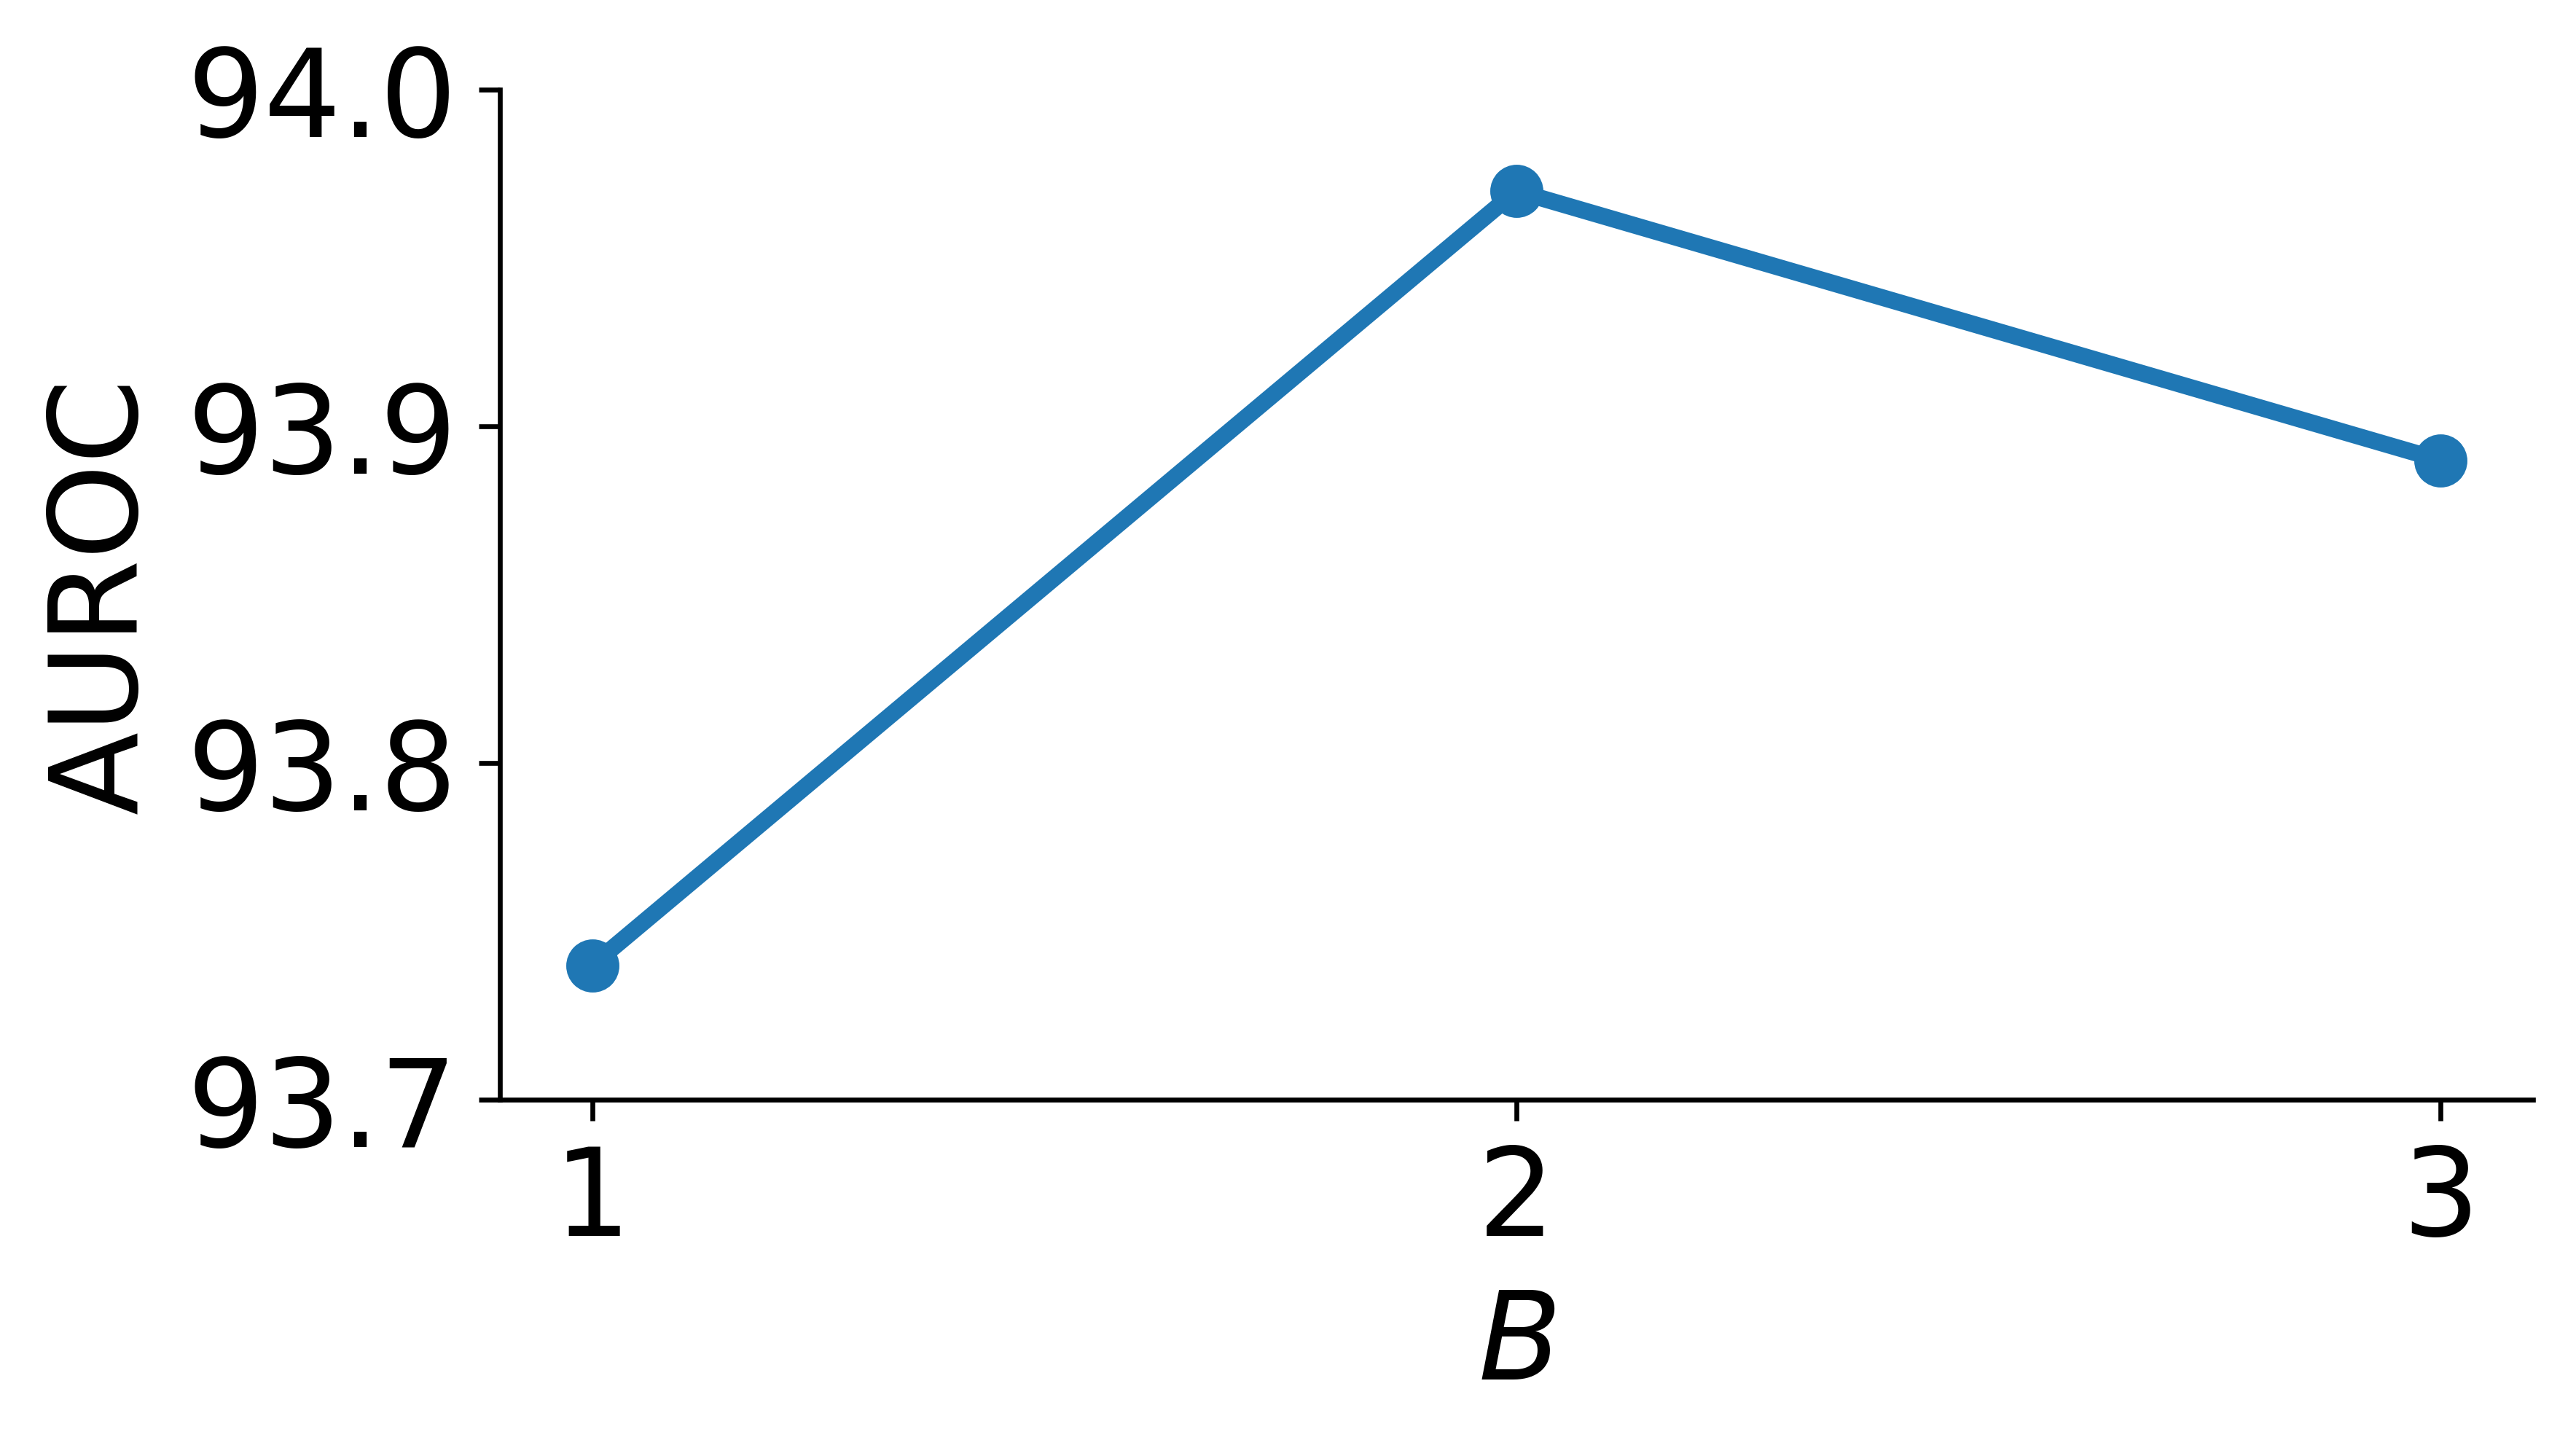
\includegraphics[width=0.55\linewidth]{figures/B_hparam_plot}
	\caption{Plot of \sys AUC against $B$.
	}
	\label{fig:blocks_hparam_plot}
\end{figure*}

%\textbf{Impact of $B$.} %To evaluate whether multi-layer cross-view feature fusion blocks (see Sec. \ref{sec:method-rep}) improve feature learning, 
%We experiment with a range of blocks $B = \{1, 2, 3\}$. Figure \ref{fig:blocks_hparam_plot} shows the average AUC trend for I-100-R ID. Using $B = 2$ blocks gives the highest AUC.% but the difference is minimal for small-scale datasets like I-100-R. %$B > 2$ blocks may be needed for more complex datasets, an investigation we leave for future research.
\subsubsection{Impact of the Number of Blocks}
The choice of number of blocks $B$ in \gls{cvca} affects the performance of \gls{sys}. To evaluate this effect on feature learning and OOD detection performance, an experiment was conducted over a range of blocks $B = \{1, 2, 3\}$. \ref{fig:blocks_hparam_plot} displays the average AUC trend for ImageNet-100 ID. $B = 2$ blocks results in the highest AUC performance from \gls{sys} but the difference is minimal for small-scale datasets like ImageNet-100. $B > 2$ blocks may be needed for more complex datasets.

\begin{table*}[htp!]
	%\small
	\centering
	\caption{ 
		Ablation OOD detection results (AUC, FPR) for ImageNet-100 ID comparing \sys to single-view models with equivalent data and equivalent parameters.%Results from 1 seed.
	}
\vspace{0.1cm}
	\scalebox{1.}{
		\begin{tabular}{|l|cccccc|}
			\hline
			%\multirow{2}{*}{} &  \multicolumn{6}{c|}{OOD}        \\ \cline{2-7} 
			%& Average (Far) & Average (Near) & Average \\ \hline
            & \multicolumn{2}{c}{Average (Far)} & \multicolumn{2}{c}{Average (Near)} & \multicolumn{2}{c|}{Average} \\ 
            & AUC$\uparrow$ & FPR$\downarrow$ & AUC$\uparrow$ & FPR$\downarrow$ & AUC$\uparrow$ & FPR$\downarrow$ \\ \hline
			Aug Base & 92.73 & 38.83 & 80.53 & 69.15 & 87.85 & 50.96  \\ 
			Fg-Bg Base & 92.70 & 38.88 & 80.51 & 69.10 & 87.83 & 50.97  \\ \cdashline{1-7}
			EqParam & 96.00 & 21.19 & 88.43 & 47.86 & 92.56 & 33.31  \\ \cdashline{1-7}
			%Rot-Noise & 95.74 & 16.06 & 87.28 & 46.06 & 90.90 & 28.06 \\
			%Crops & 95.74 & 19.87 & 87.40 & 45.44 & 90.97 & 30.10  \\  \hdashline
			\gls{sys} & 97.39 & 13.38 & 89.68 & 47.84 & 93.89 & 29.04  \\ \hline
		\end{tabular}
	}
	\label{tab:moredata_ablations_aug}
\end{table*}


%{\color{blue}
%\subsection{Comparison with Equivalent Data and Parameters}
%\label{sec:suppmat-eqparam}

%\textbf{Equivalent Augmented Data and Parameters.} One can argue that the comparison of \sys 
%with existing OOD baselines is unfair due to baselines 1) only using the original image while \sys uses the original image and its foreground and background views, and {\color{blue}2) having fewer learnable parameters than \sys}. %We note that this is an \textit{inherent property} of our proposed exploration, as we exploit multiple views for OOD detection performance benefits and design an effective framework to leverage it. Also, here, the additional views are generated automatically with an off-the-shelf toolkit and involve no explicit data collection effort. Furthermore, it has been shown that simply providing more data may not be enough in solving the OOD detection problem \cite{fang2022out}, attesting to the necessity of principled techniques such as \sys.
%Recent theoretical results show that simply providing more data is not enough to solve the OOD detection problem \cite{fang2022out}, attesting to the necessity of principled techniques such as \sys and establishing comparability between \sys and baselines. %Furthermore, our problem domain of using multiple views \textit{inherently necessitates more data} which we demonstrate can be efficiently processed with an off-the-shelf toolkit.
%
%%Despite this, we conducted two experiments where the baseline model is provided with the original image and two additional augmented images per sample to equalize the amount of training data between baselines and \sys. The augmentations chosen for the first experiment were based on findings indicating their benefit for OOD detection and include \textit{rotations} (from CSI \cite{tack2020csi}) and \textit{noise} (from random augmentation works \cite{cubuk2020randaugment}). %,hendrycks2022pixmix}). 
%%For the second experiment, we use the foreground and background views as the additional augmented images. The OOD detection results of these experiment on ID dataset I-100-R are presented in Table \ref{tab:moredata_ablations_aug} in rows ``Aug Base'' and ``Fg-Bg Base'' respectively. We chose the best-performing baseline OOD detection method, ViM, for comparison. \sys still outperforms baselines trained with equivalent data, showing that (1) cross-attention fusion of foreground-background views is key to improve OOD detection with segmented images, and (2) %our proposed \sys framework can effectively utilize such views, whose 
%%\sys performance benefits do not come from additional data. {\color{blue}We further consider the comparison between \sys and baseline models with equivalent number of parameters in Table \ref{tab:moredata_ablations_aug} (row ``EqParam'') and Appendix Sec. {\color{red}TODO}. \sys outperforms equivalent parameter baselines, showing the importance of CVCA fusion of multiple views.}
%We conduct experiments where the baseline model is 1) provided with two additional images per sample to equalize the amount of training data, and {\color{blue}2) provided the same number of parameters as \sys}. Results of these experiment on I-100-R ID are in Table \ref{tab:moredata_ablations_aug} in rows ``Aug Base'' (augmentations of the original image), ``Fg-Bg Base'' (segmented images used in \sys), and {\color{blue}``EqParam''. Details for the experiments are in Appendix Sec. E.3.} \sys still outperforms the baselines, showing that \sys performance gains do not come from additional resources and cross-attention fusion of foreground-background views is key to improve OOD detection with segmented images. %our proposed \sys framework can effectively utilize such views, whose 
%%.% {\color{blue}We further consider the comparison between \sys and baseline models with equivalent number of parameters in Table \ref{tab:moredata_ablations_aug} (row ``EqParam'') and Appendix Sec. {\color{red}TODO}. \sys outperforms equivalent parameter baselines, showing the importance of multiple view fusion.}
%
%Here we detail the experiments evaluating the performance of single-view baseline models when provided data and learnable parameters equivalent to those provided to \sys.
%
%\textbf{Equivalent Data.} Two experiments were conducted where the baseline model was provided with the original image and two additional augmented images per sample to equalize the amount of training data between baselines and \sys. The augmentations chosen for the first experiment were based on findings indicating their benefit for OOD detection and include \textit{rotations} (from CSI \cite{tack2020csi}) and \textit{noise} (from random augmentation works \cite{cubuk2020randaugment}). %,hendrycks2022pixmix}). 
%For the second experiment, we use the foreground and background views (used in \sys) as the additional augmented images. The OOD detection results of these experiment on ID dataset ImageNet-100-Random are presented in main paper Table 5 in rows ``Aug Base'' and ``Fg-Bg Base'' respectively. We chose the best-performing baseline OOD detection method, ViM, for comparison. \sys consistently outperforms baselines trained with equivalent data. This implies that the CVCA in \sys is key to improve OOD detection through fusion of the segmented foreground-background images. Furthermore, \sys performance benefits do not come from additional data.
\subsubsection{Comparison with Equivalent Data and Parameters}
\label{sec:suppmat-eqparam}
\gls{sys} utilizes multiple views of an image to perform OOD detection. A natural concern is that the performance of \gls{sys} is due to the use of additional data (three views as input instead of only one input, i.e. the original image) and additional parameters (three feature extractors and $\mathcal{U}$). This concern is unfounded because the problem inherently demands a different comparison. The nature of the multi-view OOD detection task implies the availability and necessary processing of additional data. The comparison to single-view baselines is out of necessity. Few previous multi-view OOD detection methods exist that are comparable to the methodology of \gls{sys}. \gls{sys}, comparatively, exploits multiple views for OOD detection by explicitly designing a framework to effectively leverage them. Furthermore, the additional views in multi-view OOD detection are not equivalent to additional data in the traditional sense presented in OOD detection literature. Each view is an augmentation of the original image and generated automatically (or already available) as part of the task setting, requiring no additional effort (e.g. data collection). Finally, it has been shown that solving the OOD detection problem fundamentally requires more than simply learning from or otherwise utilizing additional data \cite{fang2022out}. It is necessary to use principled techniques such as \gls{sys} in the presence of data to achieve state-of-the-art OOD detection, especially in the near-OOD domain.

Despite this, two additional experiments were conducted to evaluate the performance of \gls{sys} relative to baselines that 1) utilized additional data, and 2) utilized additional trainable parameters.
For the first experiment, a single-view baseline model was provided with two additional augmented images per sample (in addition to the original image), establishing an equal amount of training data between the baseline and \gls{sys} (Aug Base in \ref{tab:moredata_ablations_aug}). The augmentations chosen were inspired by established OOD detection works and include rotations (from CSI \cite{tack2020csi}) and noise (from random augmentation methods \cite{cubuk2020randaugment}). Additionally, a single-view baseline model was provided with the foreground and background segmented views along with the original view (Fg-Bg Base in \ref{tab:moredata_ablations_aug}). OOD detection results for \gls{sys} against these equivalent-data baseline for ImageNet-100 ID are in \ref{tab:moredata_ablations_aug}. Baselines used VIM. \gls{sys} outperforms baselines trained on equivalent data. This affirms that the performance increase with \gls{sys} is not from additional data but from an intelligent utilization of segmented views via \gls{cvca} fusion for OOD detection.

%{\color{blue}
%\textbf{Equivalent Parameters.} Another claim could be that \sys outperforms existing baselines due to the increase in parameters. To empirically verify that this is not the case, we conduct an experiment with a version of the single-view baseline model containing learnable parameters equivalent to those in \sys (i.e. 48M). The results on I-100-R ID are shown in Table \ref{tab:moredata_ablations_aug}. Even with more parameters, the baselines do not outperform \sys, indicating that the view fusion mechanisms introduced by \sys are critical to improved performance instead of the parameter increase. {\color{red}move to Appendix and explain why this difference doesn't matter, models will have different sizes, changing pretrained model/backbone is very unfair - our method proposed the FF not the backbone, we still outperform; MAKE SURE THIS IS IN THE REBUTTAL AS WELL}
%}
%
%\textbf{Equivalent Parameters.} Another claim could be that \sys outperforms existing baselines due to the increase in parameters. To empirically verify that this is not the case, we conduct an experiment with a version of the single-view baseline model containing learnable parameters equivalent to those in \sys (i.e. 48M). The results on ID dataset ImageNet-100-Random are shown in main paper Table 5. Even with more parameters, the baselines do not outperform \sys, indicating that the view fusion mechanisms introduced by \sys are critical to improved performance instead of the parameter increase.
%
%We note that changing the feature extraction backbone for the single-view baseline (i.e. by increasing the number of learnable parameters) but not for \sys is an unfair comparison. A significant amount of the learnable parameters (28.67 MiB) in \sys are in the feature fusion head, which is designed to be modular to patch-based feature extraction backbones. The intuitive decision when presented with a superior feature extraction backbone would be to use it with our proposed feature fusion head, thus re-establishing a fair comparison with \textit{equivalent feature extractors}. Nevertheless, \sys still outperforms the single-view baseline with equivalent parameters despite using weaker feature extraction backbones. %{\color{red}move to Appendix and explain why this difference doesn't matter, models will have different sizes, changing pretrained model/backbone is very unfair - our method proposed the FF not the backbone, we still outperform; MAKE SURE THIS IS IN THE REBUTTAL AS WELL}
%}
For the second experiment, a single-view baseline model was expanded in each layer dimension such that the final trainable parameter count was equivalent to those in \gls{sys} (i.e. 48M). The results comparing OOD detection performance between \gls{sys} and the equivalent-parameter baseline on ImageNet-100 ID are in \ref{tab:moredata_ablations_aug} (EqParam row). Despite the additional parameters available to the single-view baseline, \gls{sys} still outperforms baseline methods. This further establishes that the performance improvements evidenced by \gls{sys} are not from an increased amount of trainable parameters. The mechanisms in \gls{sys}, such as leveraging of multi-view data and CVCA feature fusion, are critical to the improved OOD detection displayed by \gls{sys}.

This comparison is additionally valuable because it reiterates an important discrepancy across ML and commonly compared against in OOD detection. Changing the sizes of feature extraction backbones in baselines, e.g. by increasing the amount of trainable parameters but not for \gls{sys}, is an illogical and irreconcilable comparison. The existence of such a backbone could be used directly in \gls{sys} as the trainable parameters and contributions of \gls{sys} are not from the feature extraction backbones (which are simply pre-trained models used directly from source). \gls{sys} uses LoRA adapters and $\mathcal{U}$ on top of such pre-trained backbones. In fact, a significant mount of trainable parameters in \gls{sys} (28.67 MiB) are in the fusion component $\mathcal{U}$, which is modular to any patch-based feature extraction backbone. Intuitively, any superior feature extraction backbone (e.g. one with increased parameters as described above) would simply be used with the LoRA adapters and $\mathcal{U}$ in a complementary relationship. Establishing a comparison between different feature extraction backbones in \gls{sys} and a baseline is both meaningless from a practical standpoint and unfair from the perspective of scientific evaluation. Nevertheless, \gls{sys} remains superior over single-view baselines despite the difference in parameters between feature extraction backbones.

%{\color{purple} The Table 5 results were included together to save space in the draft. We will separate the Aug Base comparison from the Split and Crops comparisons in our revision. We further evaluated baselines with the suggested foreground and background augmentations and found them to be weaker than COD. Results are below and we will include them in our revision. Experiment setting is ImageNet-100-Random.
%	
%	Fg-Bg Baseline: 80.51\%, 92.70\%, 87.83\% \\
%	COD (ours): 89.07\%, 97.24\%, 93.97\% \\
%}

%\begin{table*}[htp!]
%	%\small
%	\centering
%	\caption{ 
%		Ablation OOD detection results (AUC, FPR) for ImageNet-100 ID for \sys with different post-hoc OOD detection methods.
%	}
%	\vspace{0.15cm}
%	\scalebox{0.9}{
%		\begin{tabular}{|l|cccccc|}
%			\hline
%		%\multirow{2}{*}{} &  \multicolumn{6}{c|}{OOD}        \\ \cline{2-7} 
%		%& Average (Far) & Average (Near) & Average \\ \hline
%        & \multicolumn{2}{c}{Average (Far)} & \multicolumn{2}{c}{Average (Near)} & \multicolumn{2}{c|}{Average} \\ 
%        & AUC$\uparrow$ & FPR$\downarrow$ & AUC$\uparrow$ & FPR$\downarrow$ & AUC$\uparrow$ & FPR$\downarrow$ \\ \hline
%			MSP & 90.77 & 49.45 & 84.77 & 65.55 &  87.77 & 57.50 \\ 
%			KNN & 93.30 & 36.66 & 75.05 & 82.37 & 84.18 & 59.52  \\ \hdashline
%			\sys-MSP & 92.60 & 35.30 & 89.01 & 48.93 & 90.07 & 41.49  \\ 
%			\sys-KNN & 95.35 & 24.38 & 88.17 & 55.83 & 92.08 & 38.67  \\ \hdashline
%			\sys & 97.31 & 13.49 & 89.16 & 47.76 &  93.24 & 30.63 \\ \hline
%		\end{tabular}
%	}
%	\label{tab:ab_othermethods}
%	\vspace{-0.1cm}
%\end{table*}
%{\color{blue}
%\subsection{Segmented Foreground-Background Quality and Domain Shift}
%\label{sec:suppmat-fgbgqualds}

%\textbf{Augmented Views.} Rotations and noise image augmentations have been shown to improve OOD detection \cite{tack2020csi,cubuk2020randaugment}. We experiment with training \sys with a rotated image and a noisy image instead of segmented views. % to investigate if such augmentations are sufficient for improved OOD detection. 
%Results for I-100-R ID are in Table \ref{tab:moredata_ablations_aug} (``Rot-Noise''). \sys with segmented views is superior to using augmentations.%, verifying the usefulness of the segmented feature information.

%\textbf{Effect of Foreground-Background Quality.} We investigate if the performance benefits of \sys are reliant on properly segmented foregrounds and backgrounds. For this, we perform two evaluations.

%%For evaluation (1), we generate two additional datasets with poor semantic correlation across views: each view contains half of the image split vertically (``Split''), and one view contains off-center crops of the image while the other view contains the rest of the image (``Crops''). Results of this experiment on ID dataset I-100-R are presented in Table \ref{tab:moredata_ablations}. %in rows ``Split'' and ``Crops''. 
%First, we evaluate \sys with improperly separated foregrounds and backgrounds. Results of this experiment on I-100-R ID are presented in Table \ref{tab:moredata_ablations_aug} in row ``Crops'' (details in Appendix Sec. E.4).
%\sys with foreground-background views outperforms poor segmentation views, indicating that \sys improves with increasingly semantically meaningful segmentation. {\color{blue}This is supported in further experiments with a weaker segmentation model (see Appendix Sec. E.5).} % for optimal discriminative feature learning and OOD detection. %\textcolor{red}{answer: why is Rot-Noise worse than Crops? shouldn't random Crops be worse?} \alex{potential reason - existing work in e.g. jigsaw augmentations gives good results for OOD detection, random crops simulates this just in two different views}
%
%We provide details for our investigation into if \sys performance benefits originate in properly segmented foregrounds and backgrounds. For this, two questions are asked:
%\begin{enumerate}
%    \item Does \sys require properly separated foregrounds and backgrounds?
%    \item Can \sys still perform well across datasets of varying separation quality?
%\end{enumerate}
%
%For (1), we generate an additional dataset with poor semantic correlation across views: one view contains off-center crops of the image while the other view contains the rest of the image (``Crops''). Results of this experiment on ID dataset ImageNet-100-Random are presented in main paper Table 5. 
%\sys with the poor segmentation-quality dataset is weaker than \sys with foreground-background segmentation. This demonstrates that increasingly semantically meaningful foregrounds and backgrounds directly improve the performance of \sys. 
%
\subsubsection{Segmented Foreground-Background Quality and Domain Shift}
\label{sec:suppmat-fgbgqualds}

An important question is if the performance benefits of \gls{sys} stem from properly segmented foreground and background views. This question is complex and requires analysis across a range of segmentation quality, both from the perspective of the segmentation procedure itself and from the perspective of domain shift.

\begin{table*}[htp!]
	%\small
	\centering
	\caption{ 
		Ablation OOD detection results (AUC, FPR) on ImageNet-100 ID using the original image and two additional synthetic views instead of foreground-background segmented views. %Results from 1 seed.
	}
\vspace{0.1cm}
	\scalebox{1.}{
		\begin{tabular}{|l|cccccc|}
			\hline
			%\multirow{2}{*}{} &  \multicolumn{6}{c|}{OOD}        \\ \cline{2-7} 
			%& Average (Far) & Average (Near) & Average \\ \hline
            & \multicolumn{2}{c}{Average (Far)} & \multicolumn{2}{c}{Average (Near)} & \multicolumn{2}{c|}{Average} \\ 
            & AUC$\uparrow$ & FPR$\downarrow$ & AUC$\uparrow$ & FPR$\downarrow$ & AUC$\uparrow$ & FPR$\downarrow$ \\ \hline
			Rot-Noise & 95.74 & 16.06 & 87.28 & 46.06 & 90.90 & 28.06 \\
			Crops & 95.74 & 19.87 & 87.40 & 45.44 & 90.97 & 30.10  \\  \cdashline{1-7}
			\gls{sys} & 97.39 & 13.38 & 89.68 & 47.84 & 93.89 & 29.04  \\ \hline
		\end{tabular}
	}
	\label{tab:moredata_ablations_views}
\end{table*}

First, the presence of properly separated foregrounds and backgrounds is evaluated using two alternative multi-view datasets with \gls{sys}. The first dataset uses the aforementioned data augmentations of rotations and noise as the ``foreground'' and ``background'' views to evaluate the performance of \gls{sys} when provided with views that are not segmented at all (Rot-Noise). The second dataset uses one view with off-center crops of the original image and the other view containing the rest of the original image (Crops). This evaluates the performance of \gls{sys} under poor semantic correlation across views. Results of \gls{sys} with these alternative multi-view datasets for ImageNet-100 ID are presented in \ref{tab:moredata_ablations_views}. \gls{sys} trained and tested on datasets with poor segmentation quality is less capable in OOD detection compared to \gls{sys} with foreground and background segmented views. This implies that \gls{sys} extracts significantly more discriminative features via \gls{cvca} from semantically meaningful foregrounds and backgrounds.

\begin{table*}[htp!]
%\small
\centering
\caption{
	Ablation OOD detection results (AUC, FPR) using ID training datasets of varying separation quality and object-domain relevance: Textures (low separation quality) and NINCO (clear separation but multiple complex objects in the foreground)
	. %Results from 1 seed. 
	Note that Textures has no known near-OOD datasets, the datasets are simply evaluated together. (b) denotes results using a baseline model.
}
\vspace{0.1cm}
\scalebox{1.}{
	\begin{tabular}{|l|cccccc|}
		\hline
		%\multirow{2}{*}{} &  \multicolumn{6}{c|}{OOD}        \\ \cline{2-7} 
		%& Average (Far) & Average (Near) & Average \\ \hline
        & \multicolumn{2}{c}{Average (Far)} & \multicolumn{2}{c}{Average (Near)} & \multicolumn{2}{c|}{Average} \\ 
        & AUC$\uparrow$ & FPR$\downarrow$ & AUC$\uparrow$ & FPR$\downarrow$ & AUC$\uparrow$ & FPR$\downarrow$ \\ \hline
		Textures (b) & \slash & \slash & \slash & \slash & 95.94 & 19.05  \\ 
		(\gls{sys}) & \slash & \slash & \slash & \slash & 96.61 & 14.73  \\ \cdashline{1-7}
		NINCO (b) & 80.62 & 60.03 & 95.65 & 20.38 & 84.37 & 50.12 \\ 
		(\gls{sys}) & 88.61 & 44.61 & 92.85 & 30.06 & 89.67 & 40.97  \\ \hline
	\end{tabular}
}
\label{tab:segqual_ablations}
\end{table*}

%Second, we evaluate \sys across datasets of varying separation quality {\color{blue}due to domain shift, i.e. when the ID and OOD data include fewer object features which the YOLOv5 segmentation model was trained on (i.e. COCO) \cite{jocher2020ultralytics}.} We select the non-ImageNet datasets of Textures, NINCO, {\color{blue}and a medical dataset} as ID datasets (details in Appendix Sec. E.4). Results in Table \ref{tab:segqual_ablations} and Appendix Sec. E.4 indicate that \sys trained with varying foreground-background separation quality {\color{blue}and domain shift} \textit{still achieves superior OOD detection performance}. This shows that \sys is robust to foreground-background quality from domain shift.  % and further that the proposed cross-view attention is critical to learning discriminative features in images. 
%%These results also show that \sys is not tightly coupled to the ID training dataset nor the segmentation tool as both Textures and NINCO are mutually exclusive to ImageNet.% and DUTS-TR.
%
%For (2), we select non-ImageNet datasets with varying foreground-background separation quality as ID data. The Textures dataset does not have clear foreground objects and we use it to evaluate \sys performance when ID training data foregrounds and backgrounds are poorly separated. Furthermore, we evaluate \sys with NINCO as ID because it includes complex samples with foregrounds containing multiple objects. With Textures as the ID dataset, we use I-30, iNaturalist, Places, NINCO, SUN, OpenImage-O, Species, SSB-HARD, and Food as OOD datasets. For Textures, \sys was trained using settings identical to those of ImageNet-100-Random. With NINCO as the ID dataset, we use I-30, SSB-HARD, and Food as near-OOD datasets and Textures, iNaturalist, Places, SUN, OpenImage-O, and Species as far-OOD datasets. We trained \sys to convergence with a LoRA rank of 16. All other training and model configurations were identical to the ImageNet-100-Random experiment settings. Results in main paper Table 7 indicate that \sys is robust to foreground-background segmentation quality during training. Despite the varying quality of features in the views, \sys still outperforms baselines and comparison points. Furthermore, the results reinforce that the proposed cross-view attention is critical to learning discriminative features in images. 
Second, the efficacy of \gls{sys} is evaluated when presented with foreground-background views of varying segmentation quality. Non-ImageNet datasets are selected and segmented into foregrounds and backgrounds. The Textures dataset was selected as a low segmentation quality dataset as it does not have clear foreground objects. This evaluates the performance of \gls{sys} when presented with poorly separated views. The NINCO dataset was selected as a medium segmentation quality dataset as it contains complex images with multiple foreground objects. This evaluates the performance of \gls{sys} when presented with views containing noisy features or spurious features in the views. For Textures as the ID dataset, I-30, iNaturalist, Places, NINCO, SUN, OpenImage-O, Species, SSB-HARD, and Food were used as OOD datasets. For NINCO as the ID dataset, I-30, SSB-HARD, and Food were used as near-OOD datasets and Textures, iNaturalist, Places, SUN, OpenImage-O, and Species were used as far-OOD datasets. For both datasets, \gls{sys} was trained using settings identical to those of ImageNet-100 with the exception of NINCO which used a LoRA rank of 16. Results for \gls{sys} with datasets of varying foreground-background separation quality are presented in \ref{tab:segqual_ablations}. \gls{sys} is robust to foreground-background segmentation quality, outperforming baselines despite the quality of the view features. This further isolates the source of performance benefits from \gls{sys} to the proposed \gls{cvca} feature fusion architecture. Given somewhat correlated foreground-background views, the feature fusion component in \gls{sys} can leverage the discriminative features within and across views to learn a feature space conducive to OOD detection.

%%{\color{red}medical data - severe domain shift}
%{\color{blue}
%\textbf{\sys under Domain Shift.} We consider the performance of \sys under domain shift, i.e. when ID and OOD data do not include objects which the YOLOv5 segmentation model was trained on (i.e. COCO) \cite{a}. Results on Textures (Table \ref{tab:segqual_ablations}) show that \sys is robust to a domain shift from objects to textures. A further evaluation on medical data (severe domain shift) shows an average AUC for \sys of 79.93\% against a baseline AUC of 79.78\%. \sys weakens under severe domain shift but still slightly outperforms the baseline. Details for this study are in Appendix Sec. {\color{red}TODO}.
%%The selected segmentation model for \sys was YOLOv5, which is trained on a dataset with 80 clear object classes (i.e. COCO) \cite{a}. However, tasks may not always involve object data, exhibiting domain shift. The results on NINCO (fine-grained objects, little domain shift) and Textures (textures with no clear objects, moderate domain shift) as ID datasets from the previous section (Table \ref{tab:segqual_ablations}) indicates that \sys is also robust to domain shift.
%
%%To further evaluate \sys under severe domain shift, we additionally experiment with a medical dataset that is very different from COCO. Details on datasets and results can be found in Appendix Sec. {\color{red}TODO}). The average AUC performance of \sys is 79.93\% while the closest baseline is 79.78\%. \sys weakens under severe domain shift but still slightly outperforms the baseline. We hypothesize that this is due to the preservation of the original view ensuring at least the learned knowledge of single-view models.
%}
%
%\textbf{Domain shift.} Segmentation quality can also be used as a basis for analysis into the performance of \sys under domain shift. The selected segmentation model for \sys was YOLOv5, which is trained on an object dataset (i.e. COCO) \cite{jocher2020ultralytics}. However, tasks may not always involve object data. We investigate the performance of \sys under \textit{domain shift}, that is when the ID and OOD data contain fewer or unclear object features. The results on NINCO and Textures as ID datasets indicates that \sys is also robust to domain shift. NINCO is similar to COCO and \sys performs well. Textures contains images of textures, not objects \cite{cimpoi2014describing}, and thus exhibits domain shift from COCO which contains 80 classes of clear objects \cite{lin2014microsoft}. \sys still performs well, although the performance gap is smaller with respect to the baseline.
%
%To evaluate \sys under severe domain shift, we additionally experiment with a medical dataset that is very different from COCO. Specifically, we use the MEL, NV, BCC, AK, and DF classes from the ISIC 2019 dataset \cite{codella2018skin} as ID and the BKL, VASC, and SCC classes from the ISIC 2019 dataset as well as 2000 randomly selected samples from the NCT dataset \cite{kather2018100} as OOD \cite{narayanaswamy2023exploring}. The average AUC performance of \sys is 79.93\% while the closest baseline is 79.78\%. \sys still slightly outperforms the baseline under severe domain shift, likely due to the preservation of the original view ensuring at least the learned knowledge of single-view models.
%}
Third, \gls{sys} is evaluated in a setting exhibiting extreme domain shift. That is, the data presented to \gls{sys}, and more specifically to the segmentation model used to generate the foregrounds and backgrounds subsequently leveraged by \gls{sys}, is completely different (i.e. drawn from a different distribution) from what was previously seen. This implies both covariate and semantic domain shifts which introduce significant deviations from learned knowledge, potentially resulting in unreliable performance. Specifically, the segmentation model used, YOLOv5, was pre-trained on a COCO, a dataset with 80 clear object classes \cite{jocher2020ultralytics}. Domain shift relative to COCO implies data with few or unclear object features.

The previous results of \gls{sys} on Textures as ID data indicate that \gls{sys} is robust to moderate domain shift, as Textures data does not contain any objects \cite{cimpoi2014describing}. To more thoroughly evaluate \gls{sys} with respect to heavy domain shift, a medical dataset was selected to test \gls{sys} with segmented data significantly different than the object data seen in COCO. The MEL, NV, BCC, AK, and DF classes from the ISIC 2019 dataset \cite{codella2018skin} were used as the ID dataset, and the BKL, VASC, and SCC classes from the ISIC 2019 dataset were used with 200 randomly selected samples from the NCT dataset \cite{kather2018100} as the OOD dataset \cite{narayanaswamy2023exploring}. Average AUC from \gls{sys} in this heavy domain shift experimental setting is 79.93\% while the closest baseline is 79.78\%. Despite the significantly modified data distributions and resulting segmented foreground-background views, \gls{sys} slightly outperforms baselines. It is hypothesized that this is due to the preservation of the information in the original image, allowing \gls{sys} to at least learn the original view features and achieve baseline OOD detection performance. This also implies that \gls{sys} may learn to ignore spurious view features if they do not contain discriminative feature information relative to the ID classes.

%{\color{blue}
%\subsection{Importance of Segmentation Model}
%\label{sec:suppmat-domshift}

%To further investigate the importance of segmentation model in \sys, we experiment with a U2-Net pre-trained on the DUTS-TR \cite{wang2017learning} dataset. We use ImageNet-100-Random for ID and Textures and NINCO for OOD. To ensure fairness, we remove all overlapping data between DUTS-TR and the ID and OOD datasets. The average AUC and FPR results for \sys with U2-Net is 83.51\% (AUC) and 63.63\% (FPR) while \sys (with YOLOv5) is 96.14\% (AUC) and 20.39\% (FPR). The older U2-Net is simultaneously slower at segmentation (taking about 0.8 seconds per image) and weaker than YOLOv5 at OOD detection. Qualitative analysis showed that U2-Net often segmented foreground objects correctly but frequently included spurious background features, thus diluting the discriminative features.
%
%Following recent trends in OOD detection literature using pre-trained vision-language models (VLMs) (e.g. CLIP \cite{radford2021learning}) \cite{miyai2024locoop,li2025synthesizing,jiang2024negative}, we investigate using the vision backbone from pre-trained CLIP as the feature extractor in \sys. The results are in Table \ref{tab:clip_ablation}. \sys with ViT and LoRA feature extractor backbones outperforms \sys with CLIP vision feature extractor backbones. \sys with LoRA adds additional learning capacity to the model, allowing it to learn to extract more discriminative features during training. Additionally, CLIP typically also uses \textit{text data} which is not considered in our domain. This simultaneously shows the reliance on CLIP-based OOD detection methods on text inputs as well as image inputs and demonstrates that VLM-based methods have certain limitations that prevent them from being directly translated to the image-only domain. Overall, we consider this to be an invalid comparison as 1) CLIP relies on text data while we do not, and 2) CLIP has likely seen some of the ID and OOD data before during pre-training, leading to information leakage. There is evidence for this in the literature, with CLIP achieving extremely high zero-shot OOD detection performance \cite{esmaeilpour2022zero}. \sys overcomes this challenge through our proposed view fusion method.
%}

%However, to more accommodate recent trends in OOD detection using VLMs, we try using the pretrained CLIP vision backbone in our method and include results in the Appendix (sec. E.5, pg. 9, start line 487). %The results on ImageNet-100-Random are below (AUROC; mean near-OOD, mean far-OOD, mean overall): 
%%\begin{itemize}
%%    \item CASOD-CLIP: 85.90\%, 93.48\%, 90.04\%
%%    \item \underline{CASOD}: 89.68\%, 97.39\%, 93.89\%
%%\end{itemize}
%CLIP underperforms compared to CASOD. We suspect this is due to the fact that our LoRA backbones in CASOD add additional learning capacity. This further shows that VLM-based OOD detection methods using CLIP make use of text data to improve performance while our proposed view fusion method is necessary in the image-only domain.
\subsubsection{Importance of Segmentation Model}
\label{sec:suppmat-altsegmod}

Expanding on the previous section, the performance of \gls{sys} with different segmentation models is considered as a natural subsequent evaluation. Instead of YOLOv5, two additional segmentation models % from varying pre-trained distributional relevance to the ID data considered by \gls{sys} 
are considered. First, a U2-Net pre-trained on the DUTS-TR dataset \cite{wang2017learning} is used. All overlapping data between the DUTS-TR dataset and ImageNet-100 setting ID and OOD datasets is removed to ensure fairness in the evaluation. As DUTS-TR is also an object dataset, the data semantic and covariate distributions are similar to that of YOLOv5. However, the U2-Net architecture is significantly older (and thus weaker) than that used by YOLOv5, resulting in a dissimilar data distribution for the resultant foreground and background views. Using ImageNet-100 for the ID dataset and Textures and NINCO for the OOD datasets, \gls{sys} results in an AUC of 83.51\% and FPR95 of 63.63\% using views from U2-Net. Compared to an AUC of 96.14\% and FPR95 of 20.39\% using views from YOLOv5, it is clear that the segmentation model (and resulting segmentation quality) impacts the performance of \gls{sys}. This follows the observations from the previous ablation studies and further illuminates the relevance of foreground-background view segmentation from the perspective of object separation quality (as embodied by the segmentation model pre-training). Furthermore, U2-Net is slower than YOLOv5, requiring about 0.8 seconds per image to perform foreground-background segmentation. Qualitative analysis of the images segmented by U2-Net revealed that foreground objects were often correctly isolated but frequently contained spurious background features. This diluted the discriminative features in views and degraded feature learning and subsequent OOD detection performance.

\begin{table*}[htp!]
	\small
	\centering
	\caption{ 
		Ablation OOD detection results (AUC) for ImageNet-100 ID between \sys with LoRA ViT feature extractor backbones and \sys with CLIP vision feature extractor backbone. %Results from 1 seed.
	}
\vspace{0.1cm}
	\scalebox{1.}{
		\begin{tabular}{|l|ccc|}
			\hline
			\multirow{2}{*}{} &  \multicolumn{3}{c|}{OOD}        \\ \cline{2-4} 
			& Average (Far) & Average (Near) & Average \\ \hline
			\gls{sys}-CLIP & 93.84 & 85.90 & 90.04  \\
			\gls{sys} & 97.39 & 89.68 & 93.89  \\ \hline
		\end{tabular}
	}
	\label{tab:clip_ablation}
\end{table*}

Recent OOD detection literature has focused on exploring the potential of pre-trained Vision Language Models (VLMs) \cite{miyai2024locoop,li2025synthesizing,jiang2024negative}, such as CLIP \cite{radford2021learning}. To account for this recent trend, \gls{sys} is additionally evaluated using the vision backbone from a pre-trained CLIP model as the feature extractor backbone (and including $\mathcal{U}$, adding LoRA to the CLIP model components is non-trivial and attempts led to significant performance decreases). The results on ImageNet-100 ID between \gls{sys} with ViT backbone and CLIP backbone (\gls{sys}-CLIP) are presented in \ref{tab:clip_ablation}. \gls{sys}-CLIP is worse than \gls{sys} in OOD detection. The embodied knowledge and additional learning capacity from the ViT backbone and LoRA components respectively enable significantly improved feature learning from \gls{sys} over \gls{sys}-CLIP which must rely more on the pre-trained abilities of the CLIP vision backbone. Importantly, CLIP is designed to leverage images and text data, but text data is not allowed in the considered OOD detection task. This reveals two observations. First, that CLIP relies on text inputs as well as image inputs for functionality, including OOD detection. Second, that CLIP-based OOD detection methods have limitations that prevent them from being translated to the image domain, which may be a negative consideration in applications. In summary, this is an invalid comparison both for the above reasons and because CLIP is pre-trained on a vast amount of data. This raises the likelihood that CLIP has already encountered some of the ID and OOD data presented during training and testing, a significant source of information leakage and a complete invalidation of scientific reliability. There is evidence for this leakage in literature, with CLIP exhibiting zero-shot OOD detection performance \cite{esmaeilpour2022zero}.

\begin{table*}[htp!]
	\small
	\centering
	\caption{ 
		Ablation OOD detection results (AUC) for ImageNet-100-Random ID between \sys and \sys when trained without individual view feature losses ($\mathcal{L}_{CE,fused}$ only). %Results from 1 seed.
	}
\vspace{0.1cm}
	\scalebox{1.}{
		\begin{tabular}{|l|ccc|}
			\hline
			\multirow{2}{*}{} &  \multicolumn{3}{c|}{OOD}        \\ \cline{2-4} 
			& Average (Far) & Average (Near) & Average \\ \hline
			$\mathcal{L}_{CE,fused}$ only & 97.05 & 88.19 & 93.50  \\
			\gls{sys} & 97.39 & 89.68 & 93.89  \\ \hline
		\end{tabular}
	}
	\label{tab:nomvloss_ablations}
\end{table*}

%We additionally investigated \sys using \textit{only} the fused feature CE loss $\mathcal{L}_{CE,fused}$, i.e. $\mathcal{L}_{CE} = \mathcal{L}_{CE,fused}$. The OOD detection AUC results for ID dataset ImageNet-100-Random are presented in Table \ref{tab:nomvloss_ablations}. Training with only the final fused feature reduces overall performance. This is primarily because including the individual view CE loss terms encourages learning of more diverse class discriminative features in each of the corresponding views. As the features in these views are different, the resulting individual view features contain more diverse discriminative information for feature fusion. This is particularly noticeable in the increase in near-OOD performance relative to far-OOD performance. Learning more discriminative features improves detection of challenging near-OOD samples, closing the gap for \sys to \textbf{4.21\%} from 5.31\% for \sys with only fused feature CE loss.
\subsubsection{Individual View Loss Contribution}
\label{sec:suppmat-nomvloss}

\gls{sys} uses a combination of a fused feature CE loss and individual view feature CE losses to learn ID class-relevant discriminative features during training (see Section \ref{sec:casod_method-train}). To investigate if these loss components are necessary, the performance of \gls{sys} when trained using only the fused feature CE loss $\mathcal{L}_{CE,\mathcal{U}}$, i.e. $\mathcal{L}_{CE} = \mathcal{L}_{CE,\mathcal{U}}$, was evaluated. OOD detection results with ImageNet-100 ID are in \ref{tab:nomvloss_ablations}. Without including the individual view feature CE losses, performance decreases. The loss terms for the individual view features encourage learning of class discriminative features in each corresponding view, increasing feature diversity at the feature fusion stage. As each view contains different information, learning within these views increases the representation of features beneficial for learning in subsequent \gls{cvca} feature fusion operations. This benefit is clear in the near-OOD performance. The gap between near-OOD and far-OOD detection using \gls{sys} with individual view feature CE losses is 4.21\% while it is 5.31\% without individual view feature CE losses. This reduction in performance discrepancy implies a reliance on individual view features for OOD detection in \gls{sys}. 

%\begin{table*}[t!]
%	\small
%	\centering
%	\caption{\textbf{OOD Results for \sys and different OOD methods}: \textit{near-OOD} detection (\textbf{AUC}) comparison between \sys using MD (\sys), \sys using MSP (\sys-MSP), and \sys using KNN (\sys-KNN). %
%	}
%	\scalebox{0.725}{
%		\begin{tabular}{|l|ccccc|c|cccccc|c|c|}
%			\hline
%			\multirow{2}{*}{} &  \multicolumn{14}{c|}{ID data: ImageNet-100-Random}  \\ \cline{2-15}
%			& I-30 & I-900  & NINCO & SSB-Hard & Food & Avg. - Near & Textures  & iNaturalist  & Places  & SUN & OpenImage-O & Species & Avg. - Far & Avg. \\ \hline
%            MSP    & 83.55 & 85.44 & 89.54 & 85.16 & 80.18 & 84.77 & 92.71 & 94.17 & 88.41 & 86.96 & 92.65 & 89.73 & 90.77 & 88.04 \\
%            KNN    & 77.32 & 78.33 & 80.57 & 73.28 & 65.76 & 75.05 & 96.10 & 80.39 & 86.74 & 80.29 & 87.80 & 77.33 & 84.78 & 80.36 \\ \cdashline{1-15}
%			\gls{sys}-MSP    & 88.06 & 90.43 & 91.09 & 88.81 & 86.64 & 89.01 & 92.63 & 95.75 & 93.57 & 90.38 & 92.69 & 90.57 & 92.60 & 90.97 \\
%			\gls{sys}-KNN        & 85.01 & 88.34 & 92.33 & 86.62 & 88.53 & 88.17 & 96.66 & 98.32 & 96.36 & 94.22 & 95.00 & 91.54 & 95.35 & 92.08 \\ \cdashline{1-15}
%			\gls{sys}    & 85.42 & 88.30 & 93.26 & 89.66 & 91.34 & 89.60 & 99.02 & 99.89 & 98.46 & 96.40 & 95.55 & 94.56 & 97.31 & 93.81 \\ \hline
%			\multirow{2}{*}{} &  \multicolumn{13}{c|}{ID data: ImageNet-200}  \\ \cline{2-15}
%			& I-100 & I-800  & NINCO & SSB-Hard & Food & Avg. - Near & Textures  & iNaturalist  & Places  & SUN & OpenImage-O & Species & Avg. - Far & Avg. \\ \hline
%			MSP           &  82.16 & 81.27 & 77.53 & 64.13 & 65.21 & 74.06 & 87.56 & 78.50 & 77.58 & 79.26 & 79.87 & 68.97 & 78.62 & 76.55 \\
%			KNN           &  81.99 & 82.82 & 83.72 & 72.69 & 72.17 & 78.68 & 95.67 & 86.53 & 92.56 & 89.17 & 89.75 & 76.90 & 88.43 & 84.00 \\ \cdashline{1-15}
%			\gls{sys}-MSP   & 89.68 & 89.99 & 89.00 & 83.23 & 88.40 & 88.06 & 92.44 & 95.43 & 93.94 & 94.53 & 92.65 & 81.28 & 91.71 & 90.05  \\
%			\gls{sys}-KNN   & 88.14 & 88.91 & 89.70 & 80.27 & 87.99 & 87.00 & 95.77 & 96.97 & 96.42 & 96.44 & 93.43 & 83.78 & 93.80 & 91.62 \\ \cdashline{1-15}
%			\gls{sys}       & 85.03 & 86.93 & 89.96 & 82.54 & 87.14 & 86.31 & 98.48 & 99.42 & 98.26 & 97.81 & 94.14 & 86.60 & 95.79 & 91.48  \\ \hline
%			\multirow{2}{*}{} &  \multicolumn{13}{c|}{ID data: ImageNet-1k}  \\ \cline{2-15}
%			&  &  & NINCO & SSB-Hard & Food & Avg. - Near & Textures  & iNaturalist  &  &  & OpenImage-O &  & Avg. - Far & Avg. \\ \hline
%			MSP           & \slash  & \slash & 78.11 & 68.94 & 72.27 & 73.11 & 85.52 & 88.19 & \slash & \slash & 84.86 & \slash & 86.19 & 79.28 \\
%			KNN           &  \slash & \slash & 82.25 & 65.98 & 76.62 & 74.95 & 91.12 & 91.46 & \slash & \slash & 89.86 & \slash & 90.81 & 81.75 \\ \cdashline{1-15}
%			\gls{sys}-MSP   & \slash & \slash & 82.20 & 71.40 & 76.09 & 76.56 & 81.56 & 90.04 & \slash & \slash & 86.71 & \slash & 86.10 & 81.33  \\
%			\gls{sys}-KNN   & \slash & \slash & 81.34 & 66.29 & 77.74 & 78.46 & 87.06 & 88.83 & \slash & \slash & 86.59 & \slash & 87.49 & 82.98 \\ \cdashline{1-15}
%			\gls{sys}       & \slash & \slash & 86.35 & 72.76 & 77.60 & 78.97 & 93.02 & 98.50  & \slash & \slash & 90.38  & \slash & 93.99 & 86.08  \\ \hline
%		\end{tabular}
%	}
%	\label{tab:table_oodmethods}
%\end{table*}
\begin{table*}[t!]
	\small
	\centering
	\caption{\textbf{OOD Results for \sys and different OOD methods}: \textit{near-OOD} detection (\textbf{AUC}) comparison between \sys using MD (\sys), \sys using MSP (\sys-MSP), and \sys using KNN (\sys-KNN). %
	}
    \vspace{0.1cm}
	\scalebox{1.}{
		\begin{tabular}{|l|ccccc|c|}
			\hline
			\multirow{2}{*}{} &  \multicolumn{6}{c|}{ID data: ImageNet-100}  \\ \cline{2-7}
			& I-30 & I-900  & NINCO & SSB-Hard & Food & Avg. - Near  \\ \hline
            MSP    & 83.55 & 85.44 & 89.54 & 85.16 & 80.18 & 84.77 \\
            KNN    & 77.32 & 78.33 & 80.57 & 73.28 & 65.76 & 75.05  \\ \cdashline{1-7}
			\gls{sys}-MSP    & 88.06 & 90.43 & 91.09 & 88.81 & 86.64 & 89.01 \\
			\gls{sys}-KNN        & 85.01 & 88.34 & 92.33 & 86.62 & 88.53 & 88.17  \\ \cdashline{1-7}
			\gls{sys}    & 85.42 & 88.30 & 93.26 & 89.66 & 91.34 & 89.60  \\ \hline
			\multirow{2}{*}{} &  \multicolumn{6}{c|}{ID data: ImageNet-200}  \\ \cline{2-7}
			& I-100-T & I-800  & NINCO & SSB-Hard & Food & Avg. - Near  \\ \hline
			MSP           &  82.16 & 81.27 & 77.53 & 64.13 & 65.21 & 74.06 \\
			KNN           &  81.99 & 82.82 & 83.72 & 72.69 & 72.17 & 78.68\\ \cdashline{1-7}
			\gls{sys}-MSP   & 89.68 & 89.99 & 89.00 & 83.23 & 88.40 & 88.06 \\
			\gls{sys}-KNN   & 88.14 & 88.91 & 89.70 & 80.27 & 87.99 & 87.00 \\ \cdashline{1-7}
			\gls{sys}       & 85.03 & 86.93 & 89.96 & 82.54 & 87.14 & 86.31 \\ \hline
			\multirow{2}{*}{} &  \multicolumn{6}{c|}{ID data: ImageNet-1k}  \\ \cline{2-7}
			&  &  & NINCO & SSB-Hard & Food & Avg. - Near \\ \hline
			MSP           & \slash  & \slash & 78.11 & 68.94 & 72.27 & 73.11\\
			KNN           &  \slash & \slash & 82.25 & 65.98 & 76.62 & 74.95 \\ \cdashline{1-7}
			\gls{sys}-MSP   & \slash & \slash & 82.20 & 71.40 & 76.09 & 76.56 \\
			\gls{sys}-KNN   & \slash & \slash & 81.34 & 66.29 & 77.74 & 78.46\\ \cdashline{1-7}
			\gls{sys}       & \slash & \slash & 86.35 & 72.76 & 77.60 & 78.97  \\ \hline
		\end{tabular}
	}
	\label{tab:table_oodmethods}
\end{table*}

\begin{table*}[t!]
	\small
	\centering
	\caption{\textbf{OOD Results for \sys and different OOD methods}: \textit{far-OOD} detection and average results (\textbf{AUC}) comparison between \sys using MD (\sys), \sys using MSP (\sys-MSP), and \sys using KNN (\sys-KNN). %
	}
    \vspace{0.1cm}
	\scalebox{0.83}{
		\begin{tabular}{|l|c|cccccc|c|c|}
			\hline
			\multirow{2}{*}{} &  \multicolumn{9}{c|}{ID data: ImageNet-100}  \\ \cline{2-10}
			& Avg. - Near & Textures  & iNaturalist  & Places  & SUN & OpenImage-O & Species & Avg. - Far & Avg. \\ \hline
            MSP    &  84.77 & 92.71 & 94.17 & 88.41 & 86.96 & 92.65 & 89.73 & 90.77 & 88.04 \\
            KNN    & 75.05 & 96.10 & 80.39 & 86.74 & 80.29 & 87.80 & 77.33 & 84.78 & 80.36 \\ \cdashline{1-10}
			\gls{sys}-MSP    & 89.01 & 92.63 & 95.75 & 93.57 & 90.38 & 92.69 & 90.57 & 92.60 & 90.97 \\
			\gls{sys}-KNN        & 88.17 & 96.66 & 98.32 & 96.36 & 94.22 & 95.00 & 91.54 & 95.35 & 92.08 \\ \cdashline{1-10}
			\gls{sys}    &  89.60 & 99.02 & 99.89 & 98.46 & 96.40 & 95.55 & 94.56 & 97.31 & 93.81 \\ \hline
			\multirow{2}{*}{} &  \multicolumn{9}{c|}{ID data: ImageNet-200}  \\ \cline{2-10}
			& Avg. - Near & Textures  & iNaturalist  & Places  & SUN & OpenImage-O & Species & Avg. - Far & Avg. \\ \hline
			MSP           &   74.06 & 87.56 & 78.50 & 77.58 & 79.26 & 79.87 & 68.97 & 78.62 & 76.55 \\
			KNN           &   78.68 & 95.67 & 86.53 & 92.56 & 89.17 & 89.75 & 76.90 & 88.43 & 84.00 \\ \cdashline{1-10}
			\gls{sys}-MSP   & 88.06 & 92.44 & 95.43 & 93.94 & 94.53 & 92.65 & 81.28 & 91.71 & 90.05  \\
			\gls{sys}-KNN   & 87.00 & 95.77 & 96.97 & 96.42 & 96.44 & 93.43 & 83.78 & 93.80 & 91.62 \\ \cdashline{1-10}
			\gls{sys}       & 86.31 & 98.48 & 99.42 & 98.26 & 97.81 & 94.14 & 86.60 & 95.79 & 91.48  \\ \hline
			\multirow{2}{*}{} &  \multicolumn{9}{c|}{ID data: ImageNet-1k}  \\ \cline{2-10}
			&  Avg. - Near & Textures  & iNaturalist  &  &  & OpenImage-O &  & Avg. - Far & Avg. \\ \hline
			MSP           & 73.11 & 85.52 & 88.19 & \slash & \slash & 84.86 & \slash & 86.19 & 79.28 \\
			KNN           &  74.95 & 91.12 & 91.46 & \slash & \slash & 89.86 & \slash & 90.81 & 81.75 \\ \cdashline{1-10}
			\gls{sys}-MSP   &  76.56 & 81.56 & 90.04 & \slash & \slash & 86.71 & \slash & 86.10 & 81.33  \\
			\gls{sys}-KNN   &  78.46 & 87.06 & 88.83 & \slash & \slash & 86.59 & \slash & 87.49 & 82.98 \\ \cdashline{1-10}
			\gls{sys}       &  78.97 & 93.02 & 98.50  & \slash & \slash & 90.38  & \slash & 93.99 & 86.08  \\ \hline
		\end{tabular}
	}
	\label{tab:table_oodmethods_f}
\end{table*}

%\section{\sys with Other OOD Detection Methods}
%\label{sec:suppmat-ood}

%%\textbf{\sys with Other OOD Detection Methods.} We test additional post-hoc OOD detection methods with \sys to evaluate generalizable performance improvements. We present the results of an experiment including \sys with MSP (\sys-MSP) and \sys with KNN (\sys-KNN) with I-100-R ID in Table \ref{tab:ab_othermethods}. \sys combined with post-hoc OOD detection methods outperform their single-view baselines, indicating the generalizable increase in performance through view fusion. Additional details on the experiment can be found in Appendix Sec. {\color{red}TODO}.
%{\color{blue}\textbf{\sys with Other OOD Detection Methods.} We test additional post-hoc OOD detection methods (MSP, KNN) with \sys to evaluate generalizability. We present the results of an experiment with I-100-R ID in Table \ref{tab:ab_othermethods}. \sys combined with post-hoc OOD detection methods outperform their single-view baselines. %, indicating the generalizable increase in performance through view fusion.
%
%\sys is directly compatible with any post-hoc OOD detection method that makes use of logits (using $\hat{y}_{fused}$) or features (using $z_{fused}^0$). We present additional OOD detection results (AUC) for ImageNet-100-Random ID, ImageNet-200 ID, and ImageNet-1k ID using OOD detection methods MSP \cite{hendrycks2017baseline} and KNN \cite{sun2022out} in Table \ref{tab:table_oodmethods}. MSP is a logits-based method and KNN is a recent highly-competitive features-based method \cite{zhang2023openood} like MD (which is presented in the main paper). We also include MD OOD detection with \sys (the original proposed method) here. \sys with MD is the best overall performer. Interestingly, \sys-MSP is slightly better for some near-OOD datasets in the ImageNet-100-Random ID and ImageNet-200 ID settings. We suspect that this is due to model overconfidence benefiting detection of near-OOD samples similar to the ID distribution. Model logits are tuned to recognizing features in ID samples but overconfidence causes slight deviations (i.e. in near-OOD samples) to reduce the MSP score. This is not the case for the ImageNet-1k ID setting which is significantly harder to overfit due to the large number of classes. MD is generally better for far-OOD datasets as it avoids model overconfidence which is known to significantly weaken far-OOD detection \cite{nguyen2015deep, hendrycks2017baseline, wei2022mitigating, lee2018simple}. We also note that \sys with MSP and KNN is also better than the baseline MSP and KNN except for in the ImageNet-1k ID setting where \sys-KNN is slightly worse. This isolated discrepancy is suspected to be due to the significantly more complicated feature space. The class-specific comparisons in MD may be critical to discriminating between similar data in this setting. Overall, this further validates the importance of principled fusion of foreground-background views in improving OOD detection performance in the proposed \sys. %\alex{need to justify why we present VIM in the main paper even though it is better here OR remove it and/or replace it with a different OOD method. The actual reason is because VIM was much worse for ImageNet-1k so we had to use MD to be consistent}
%
%
%%Additional details on the experiment are in Appendix Sec. D.}
\subsubsection{Other OOD Detection Methods}
\label{sec:suppmat-ood}

As \gls{sys} is designed to input multi-view data and learn a feature space, outputting both a feature vector $z_{\mathcal{U}}$ and logits $\hat{y}_{\mathcal{U}}$, it is compatible with any post-hoc OOD detection method that uses those outputs. Additional OOD detection results (AUC) for the ImageNet-100 ID, ImageNet-200 ID, and ImageNet-1k ID settings using MSP \cite{hendrycks2017baseline} and KNN \cite{sun2022out} with \gls{sys} are presented in \ref{tab:table_oodmethods} for near-OOD datasets and \ref{tab:table_oodmethods_f} for far-OOD datasets and average performance. These methods cover the range of traditional OOD detection methods, with MSP being a logits-based method and KNN being a state-of-the-art feature-based method (see Chapter \ref{diss_bkgd}). Note that \gls{sys} is presented using MD in Section \ref{sec:propwork-casod-exp}. \gls{sys} with MD performs better than either MSP and KNN on average.

Additional interesting behavior can be noted from the results. \gls{sys} with MSP (\gls{sys}-MSP) performs better for some near-OOD datasets in the ImageNet-100 ID and ImageNet-200 ID settings. This is likely due to the lower difficulty of the settings. %Ordinarily a negative feature of ML, in this case it benefits \gls{sys}-MSP by strongly reinforcing the detection of near-OOD samples through inflated logits values. As model logits are trained to recognize ID features, overfitting causes the model to be hyper-sensitive to ID data and harshly penalizes even small deviations in the feature distribution, i.e. exactly those slight deviations exhibited by near-OOD data. This observation is not present in the ImageNet-1k ID setting as it is difficult to overfit the data due to the significantly larger dataset size and number of classes. 
Model logits are accurately learned for ImageNet-100 ID and ImageNet-200 ID as there are fewer classes to handle. The feature space can be ignored in favor of the accurately learned logits based on discriminative features, which increases the quality of the logits for MSP. This also explains the performance discrepancy in ImageNet-1k ID as it is much more difficult to learn discriminative features and logits in the 1000-class setting. MD and KNN generally perform better with increasing ID class space complexity.
The reason MD generally outperforms the other methods is due to its independence from model overconfidence. As model overconfidence is known to weaken far-OOD detection \cite{nguyen2015deep,hendrycks2017baseline,wei2022mitigating,lee2018simple}, avoiding this issue enables \gls{sys} to increase far-OOD detection performance along with near-OOD detection performance and achieve state-of-the-art average performance.

\gls{sys}-MSP and \gls{sys}-KNN additionally outperform their single-view baseline counterparts (i.e. MSP and KNN), with the exception being in the ImageNet-1k ID setting where \gls{sys}-KNN is slightly worse. The explanation for this discrepancy is due the the significantly more complicated feature space, resulting from the aforementioned properties of this setting. The class-specific comparisons utilized by MD are critical in discriminating between near-OOD data as it acts as an additional source of information conditioning the detection process with a targeted group of ID data. Overall, \gls{sys} is robust to OOD detection method and results further verify that \gls{sys} learns a discriminative feature space conducive to OOD detection.

%\section{Conclusion}
%\label{sec:conc}
%We present the first image-separation-based OOD detection model using foreground-background views and cross-view correlation attention feature fusion. Cross-view correlation attention fusion is a novel method that integrates feature information between the original view and the foreground and background views. The resulting fused feature space is semantically informative and improves OOD detection. Experiments show that \sys improves AUC and FPR
%across a range of near- and far-OOD datasets. 
%
%The main limitation of our work is that \sys is limited to only foreground and background views, while many images contain varying semantic objects. Our future work will study OOD detection with semantic segmentation views.
\subsubsection{Takeaways} 
\gls{sys} represents the culmination of OOD detection using foreground and background segmented images. Through the use of the proposed \gls{cvca} feature fusion architecture, discriminative features are effectively learned and applied to OOD detection in challenging experimental spaces representative of near-OOD settings and real-world applications. Furthermore, \gls{sys} leverages techniques, such as pre-trained models and LoRA Adapters, that greatly increase efficiency over equivalent models and methods. Combined with the usage of efficient segmentation models, \gls{sys} embodies an OOD detection solution that steps towards the requirements of realistic, open-world applications.

%\section{Additional Results}
%\label{sec:suppmat-results}
%
%\section{Further Analysis of \sys}
%\label{sec:suppmat-ablations}

%\textbf{Theoretical Analysis} We propose the following theoretical analysis. Self-attention applies a softmax to the features during computation of the attention matrix $A_{SA} \approx \text{softmax}(z W_{Q} W_{K}^{\intercal} z^{\intercal})$. The resultant attention matrix $A_{SA}$ consists of $3T$ rows of distributions over $3T$ patches $A_{SA} \in \mathbb{R}^{3T \times 3T}$, each with values that must be $[0, 1]$, $A_{SA,i} = \{[p_1, p_2, \dots, p_{3T}] ; p \in [0,1]\}$. CASOD uses a sum of two cross-attention matrices in each CVCA block $A_{CVCA} \approx \text{softmax}(z_{v1} W_{Q,v1} W_{K,v2}^{\intercal} z_{v2}^{\intercal}) + \text{softmax}(z_{v2} W_{Q,v2} W_{K,v1}^{\intercal} z_{v1}^{\intercal})$. The resultant CVCA attention matrix $A_{CVCA}$ is instead $T$ rows of values over $T$ patches $A_{CVCA} \in \mathbb{R}^{T \times T}$, but each value has magnitude in $[0, 2]$, $A_{CVCA,i} = \{[p_1, p_2, \dots, p_T] ; p \in [0,2]\}$.
%
%If we consider a particular high-activation patch $T^*_j \in z$ in the original image that is also in the foreground view $T^*_{fg,j} \in z_{fg}$, self-attention \textit{reduces} the magnitude of both patch activations via the softmax over all $3T$ patches. Meanwhile, our CVCA method \textit{additively reinforces} them. Both SA and CVCA optimize towards the same objective, incentivizing the attention matrices to highlight these high-activation patches. Necessarily, this requires $W_{Q}$, $W_{K}$, and $W_{V}$ to also highlight these patches, which is behavior observed in literature \cite{yeh2023attentionviz,salehi2021unified}. Given this preservation of high-activation patches into the attention matrix, the denominator of the softmax in SA is greater than the denominator of the softmax in each CVCA term
%\begin{equation}
%    \sum_{j=1}^{3T} e^{a_{SA,j}} > \sum_{j=1}^{T} e^{a_{CVCA,j}}.
%\end{equation}
%This implies 
%\begin{equation}
%    T^*_{j,CVCA} \geq T^*_{j,SA},
%\end{equation}
%where $T^*_{j,CVCA} \in A_{CVCA} z_{v1} W_{V,v1}$ and $T^*_{j,SA} \in A_{SA} z W_{V}$ are the high-activation patches of interest in the features from the attention blocks. 
%}
